\documentclass[10pt,a4paper]{article}
\usepackage[utf8]{inputenc}
\usepackage[parfill]{parskip}
\usepackage[section]{placeins}
\usepackage{graphicx}
\usepackage{array}
\usepackage{tabularx}
\usepackage{apacite}
\usepackage{url}
\usepackage[left=3.00cm, right=3.00cm, top=3.00cm, bottom=3.00cm]{geometry}

\author{Christoph Emunds (i6146758)\\Richard Polzin (???)}
\title{Information Retrieval and Text Mining\\Emotion Mining and Topic Extraction on Lyrics}
\date{\today}

\begin{document}
	\maketitle
	
	\tableofcontents
	
	\section{Introduction}
	\label{sec:introduction}
	Leaving melody aside, there is a lot of information that can be extracted from a song's lyrics. In this work, we aim to measure the similarity of artists with respect to emotions and topics of their songs based on their lyrics.
	
	In Section \ref{sec:dataset}, we give an overview over our dataset and explain how it was gathered. Section \ref{sec:preprocessing} describes the preprocessing that has been done. We mention the tools we used for the visualization in Section \ref{sec:visualization}, followed by the actual emotion mining in Section \ref{sec:emotionmining} and the topic extraction in Section \ref{sec:topicextraction} and the visualization of their results. All of the processing is done in Python 3.6.

	\section{Dataset}
	\label{sec:dataset}
	%100 top Billboard artists
	%20 metal bands from got-djent.com
	The \textit{pylyrics3} package is able to download the lyrics for all songs of a given artist if it exists on \textit{lyrics.wikia.com}. The lyrics are returned in a dictionary, where the keys are the song names and the values are the songs' lyrics. The usage of this package is straightforward and removes the necessity to deal with the raw HTML data. The retrieved songs are stored in JSON format, each song having a title, the artist's name and the actual lyrics.
	
	Some (how many?) of the top 100 Billboard artists could not be resolved when querying pylyrics3. This could be due to spelling variations. Moreover, we scraped the names of 30 metal bands from got-djent.com and requested their lyrics via pylyrics3. Some (how many?) of them could also not be resolved, either due to spelling variations or because they are not famous enough to have an entry in die LyricsWiki. Altogether, we ended up with 11.??? songs from 120 artists.

	In addition to the dataset we gathered ourselves we were given a database of more than 16.000 artists and 228.000 originally built by Sibirtsev and Schuster (???). In the remainder of this document, we call this dataset ???
	
	Some of the lyrics are not very clean. For example, they contain markers for the chorus and the verse part...

	\section{Preprocessing}	
	\label{sec:preprocessing}
	For tokenization and stemming, the \textit{nltk} Python package has been used. It provides easy to use function for splitting a document into sentences and splitting the sentences in words. Furthermore it implements several stemming algorithms. In our implementations, we use the Porter algorithm. We downloaded a list of stopwords that are more appropriate for lyrics. Moreover, in the process of topic extraction, we iteratively added words to this stopword list whenever we found...
	
	The tf-idf features are built with the help of the \textit{sklearn} package. It offers the \textit{TfIdfVectorizer} class, which...
	
	For the topic extraction, all songs should be in the same language, since otherwise the used algorithm will create an extra topic for every language.
	
	In our dataset, all songs, except for one, are in English. For the ??? dataset, we implemented a rudimentary language detection using the \textit{langdetect} Python package \cite{langdetect}. This package is a port of Google's language detection library.
	
	\section{Visualization}
	\label{sec:visualization}
	To visualize our results, we use the open-source platform \textit{Gephi}, which is able to display a plethora of graphs and networks that can also be explored interactively. Gephi provides a rich set of features. Some of the features we make use of include filtering out edges with low weight, calculating modularity classes for the nodes in a graph, ...
	
	% A bit blabla about the problems we came across, since I think we might fall short to reach the page limit
	To be able to import our results to Gephi, we made use of the \textit{pygraphml} Python package. It provides a couple of methods to dump the extracted information into a \textit{GraphML} file, that can be imported by Gephi. However, the pygraphml package is very rudimentary. An issue was that the weight attribute that has been added to edges is stored as a string, rather than a number, which makes it impossible for Gephi to recognize the edge weight properly. We circumvented this problem by simply exchanging a single line in the beginning of the GraphML file.
	
	\section{Emotion Mining}
	\label{sec:emotionmining}
	The emotion mining is done by first tokenizing every song's text. Afterwards, every token is looked up in an emotion lexicon for its emotional value. For our experiments, we used the \textit{NRC Emotion Lexicon} (EmoLex) by... This lexicon specifies the emotional value for the eight emotions \textit{anger}, \textit{anticipation}, \textit{disgust}, \textit{fear}, \textit{joy}, \textit{sadness}, \textit{surprise}, and \textit{trust}.
	
	The emotion mining we apply to the lyrics is only rudimentary, as it does not handle negations. We were not able to find an emotion lexicon that specifies the opposite emotional value for every common emotion word.
	
	After we acquired the eight dimensional emotion vector for every song, the vectors for all songs of an artist have been summed up and normalized. The resulting vectors contain information about how strong each of the eight emotions is for a certain artist. Furthermore, when calculating the distance from one artist's emotion vector to the emotion vector of every other artist, we are able to see the emotional similarity between the artists. For our experiments, we used the cosine distance as it...
	
		\subsection{Results}
		Figure \ref{fig:emotiongraph} shows a graph of all 120 artists, where each artist is connected to every emotion. The edges themselves have weights depending on the strength of the emotion in an artist's song. The weights are normalized between 0 and 1.
		
		The full graph is of course quite confusing and does not yield any useful insight. Therefore, Figure \ref{fig:reducedemotiongraph} shows a graph that contains only those edges with weights higher than $0.3$. % TODO: Explain why 0.3
		
		\begin{figure}[htb]
			\centering
			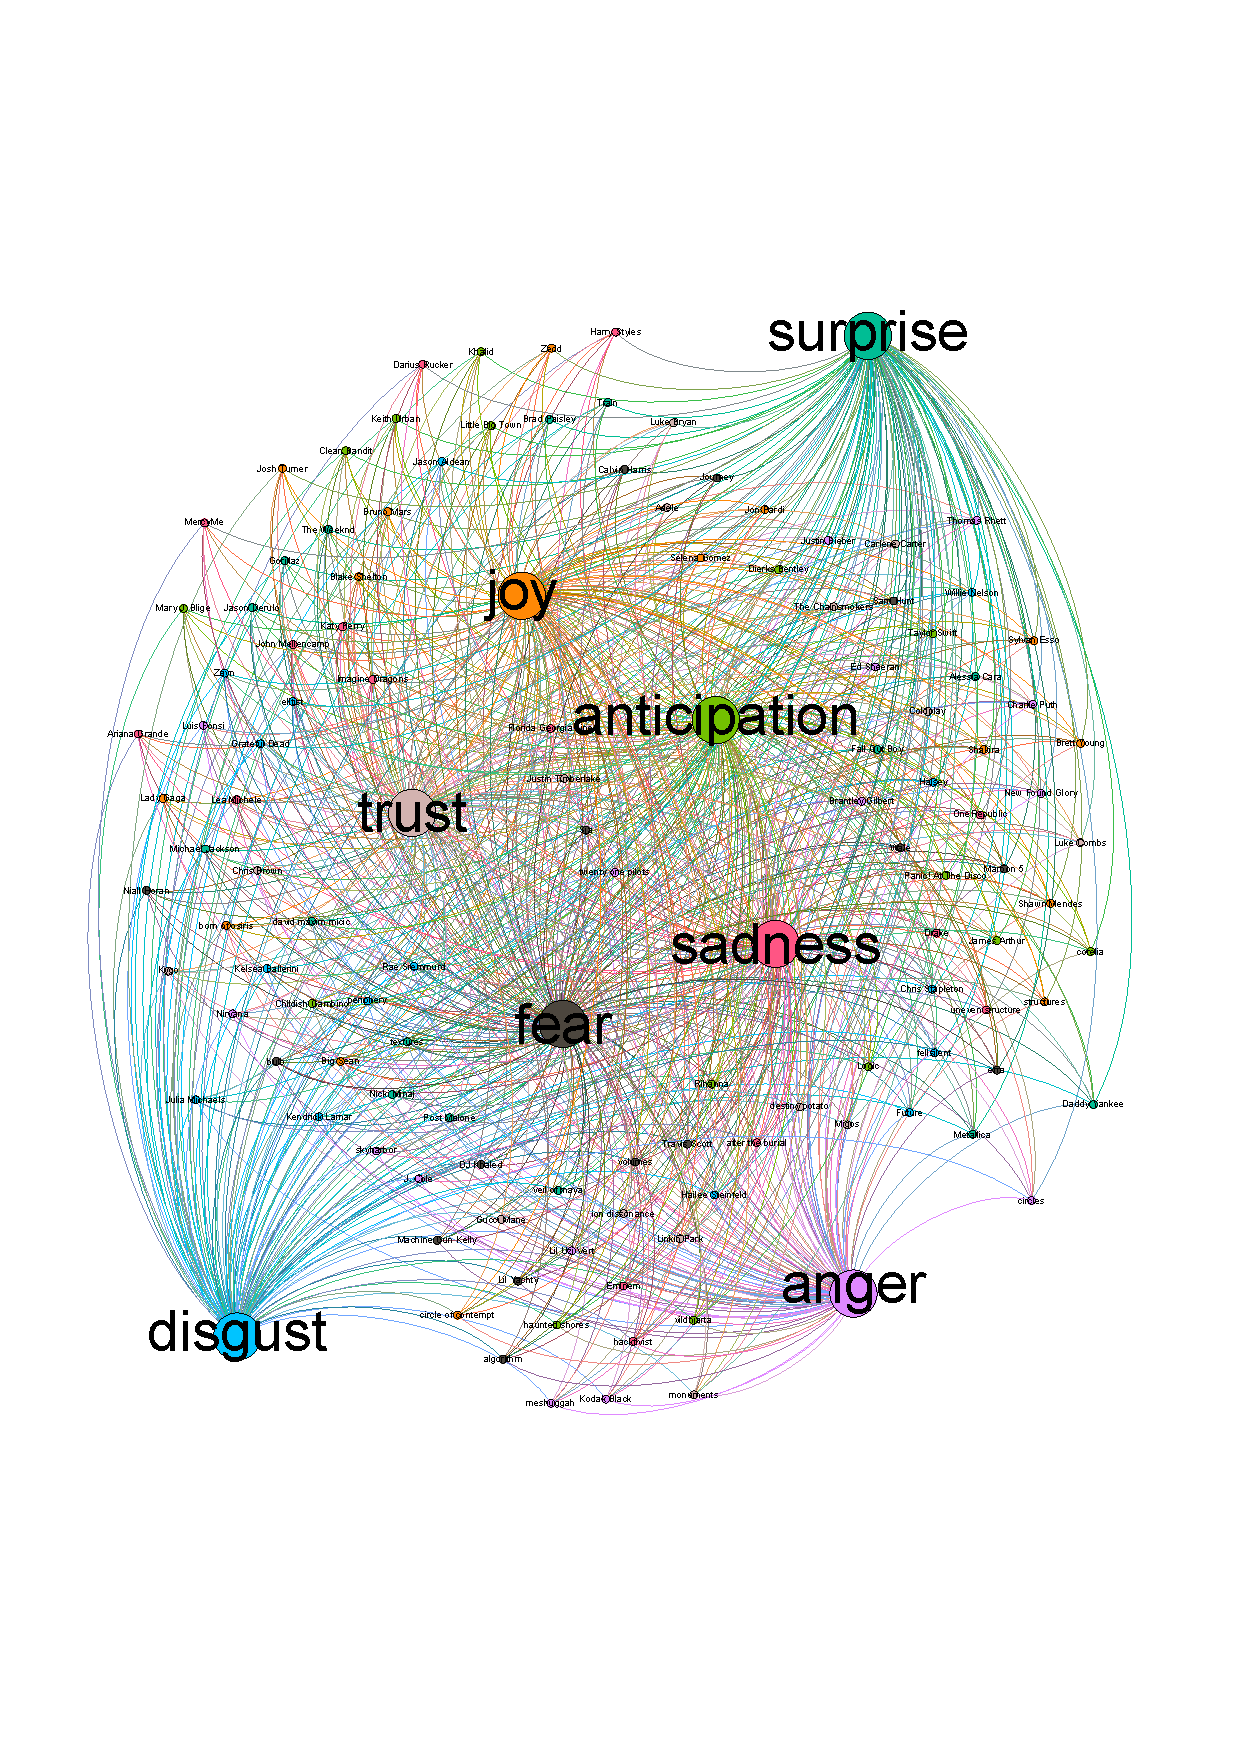
\includegraphics[trim=0mm 50mm 0mm 50mm, clip, width=0.7\linewidth]{data/emotion_graph}
			\caption{Full emotion graph}
			\label{fig:emotiongraph}
		\end{figure}
		
		\begin{figure}[htb]
			\centering
			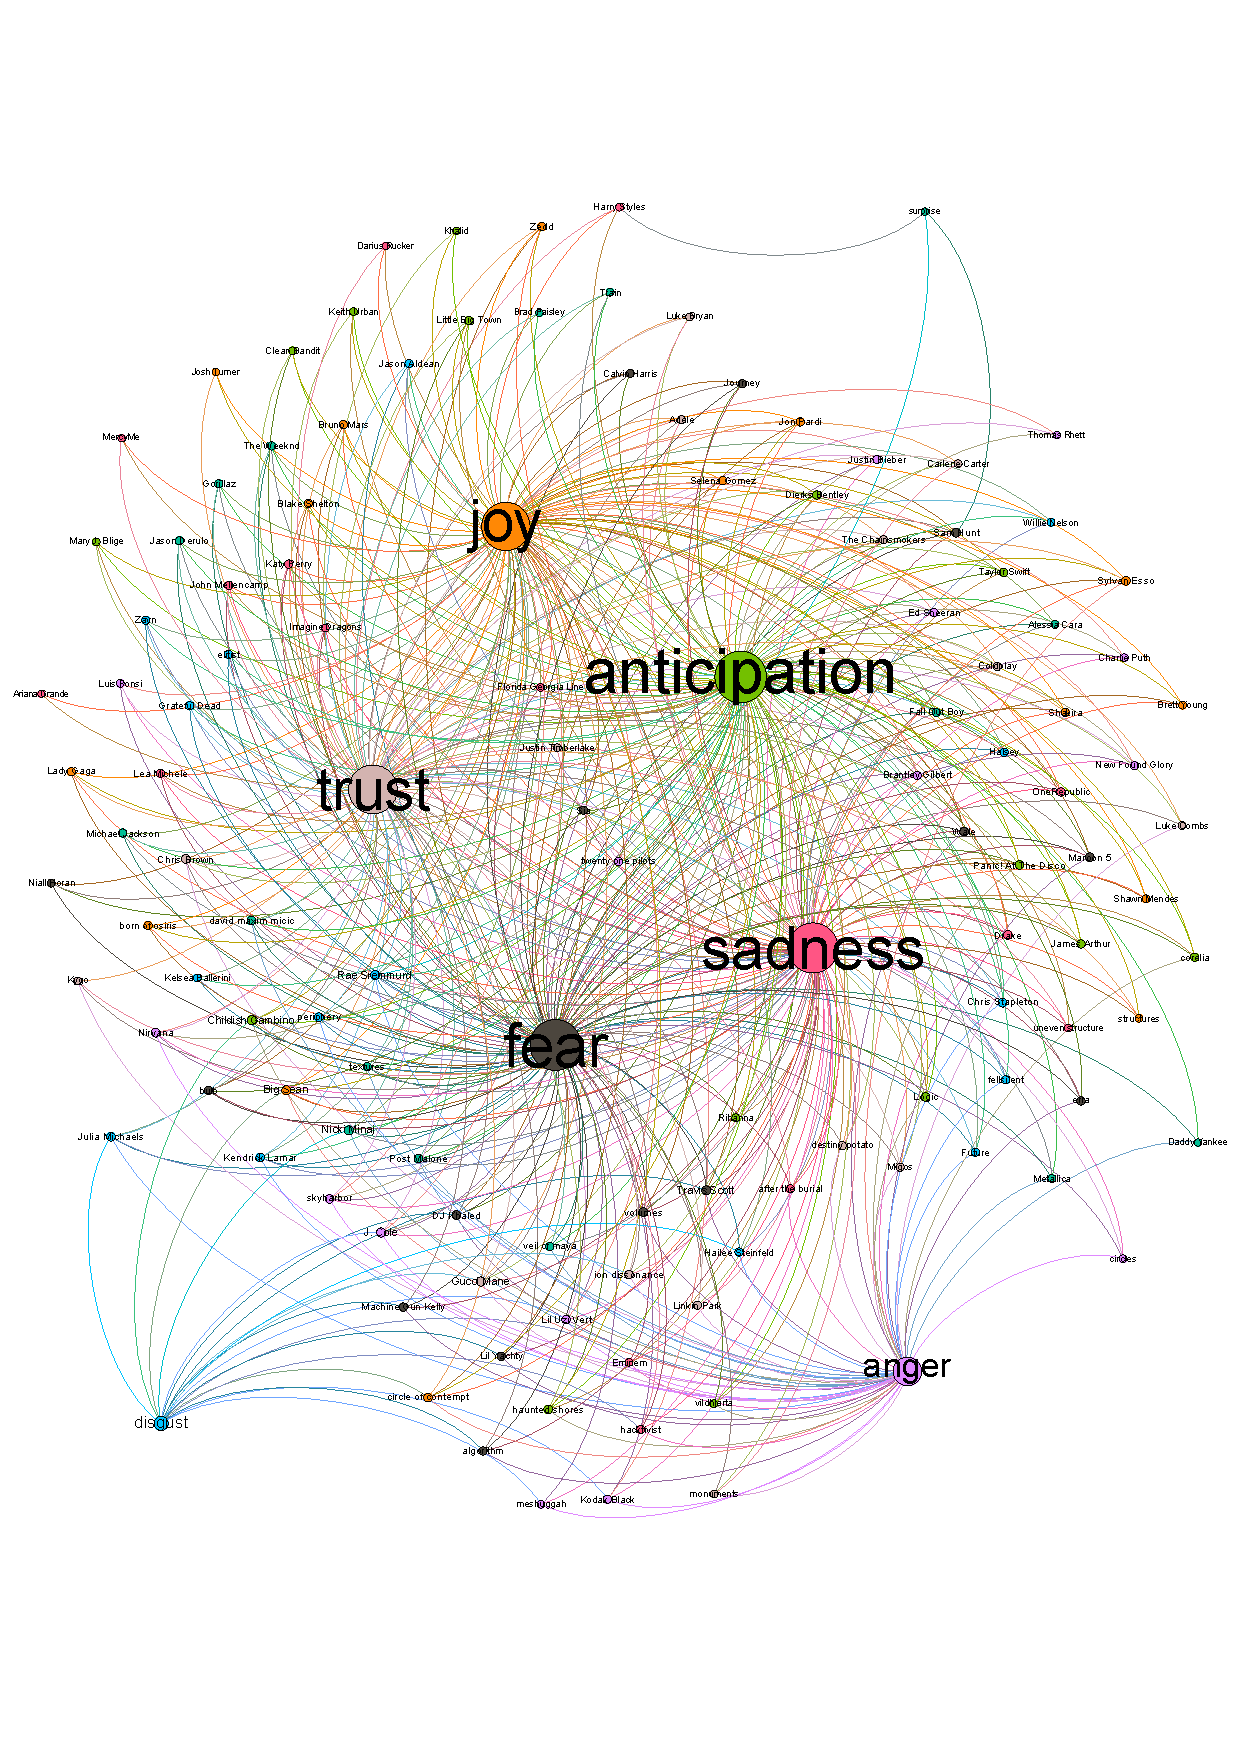
\includegraphics[trim=0mm 50mm 0mm 30mm, clip, width=0.7\linewidth]{data/emotion_graph_weight3-7}
			\caption{Emotion graph with edge weights higher than $0.3$}
			\label{fig:reducedemotiongraph}
		\end{figure}
		
		\begin{figure}[htb]
			\centering
			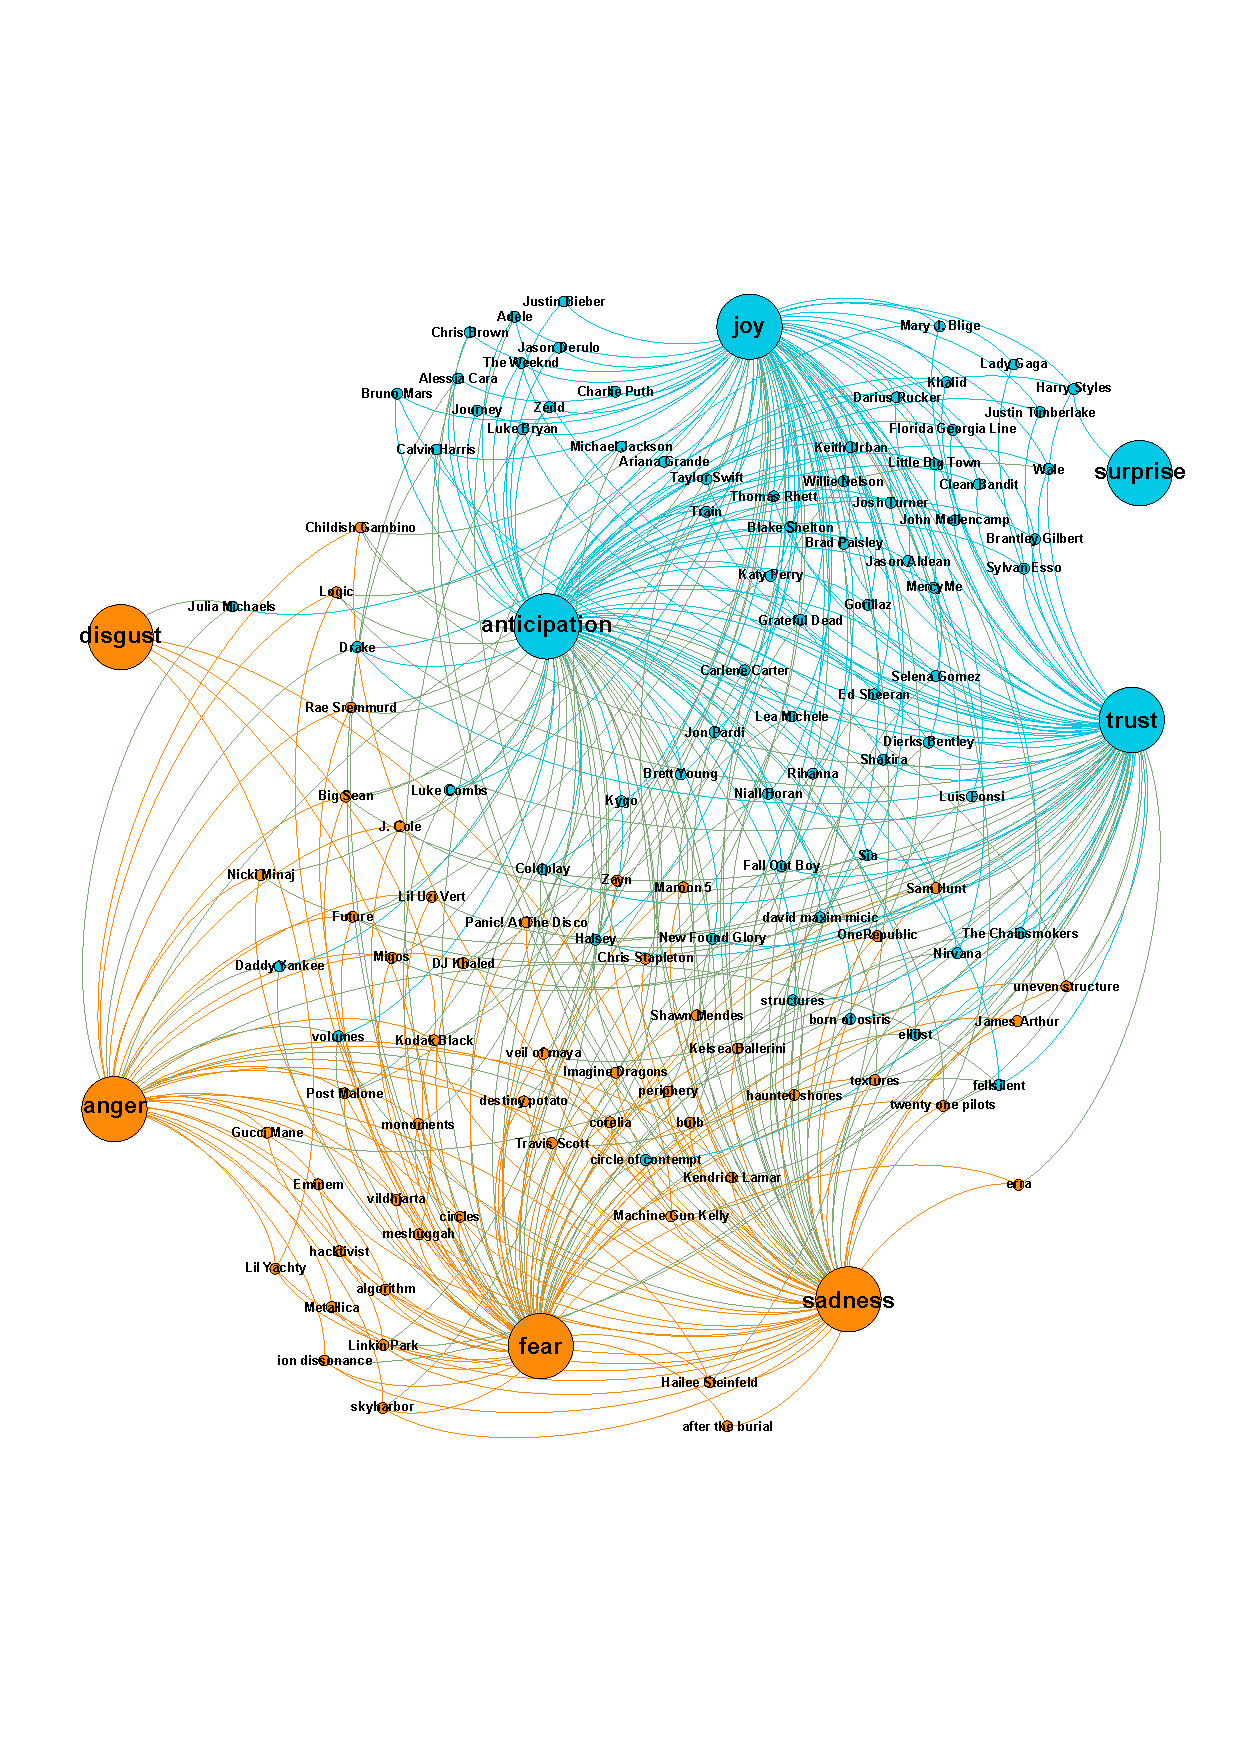
\includegraphics[trim=0mm 50mm 0mm 30mm, clip, width=0.7\linewidth]{data/emotion_graph_new_modularity}
			\caption{Reduced emotion graph with recalculated modularity}
			\label{fig:emotionnewmod}
		\end{figure}
		
		Figure \ref{fig:emotionsimilarity} shows the emotion similarity between individual artists. The modularity score separates the graph into three main regions, which...
		
		\begin{figure}[htb]
			\centering
			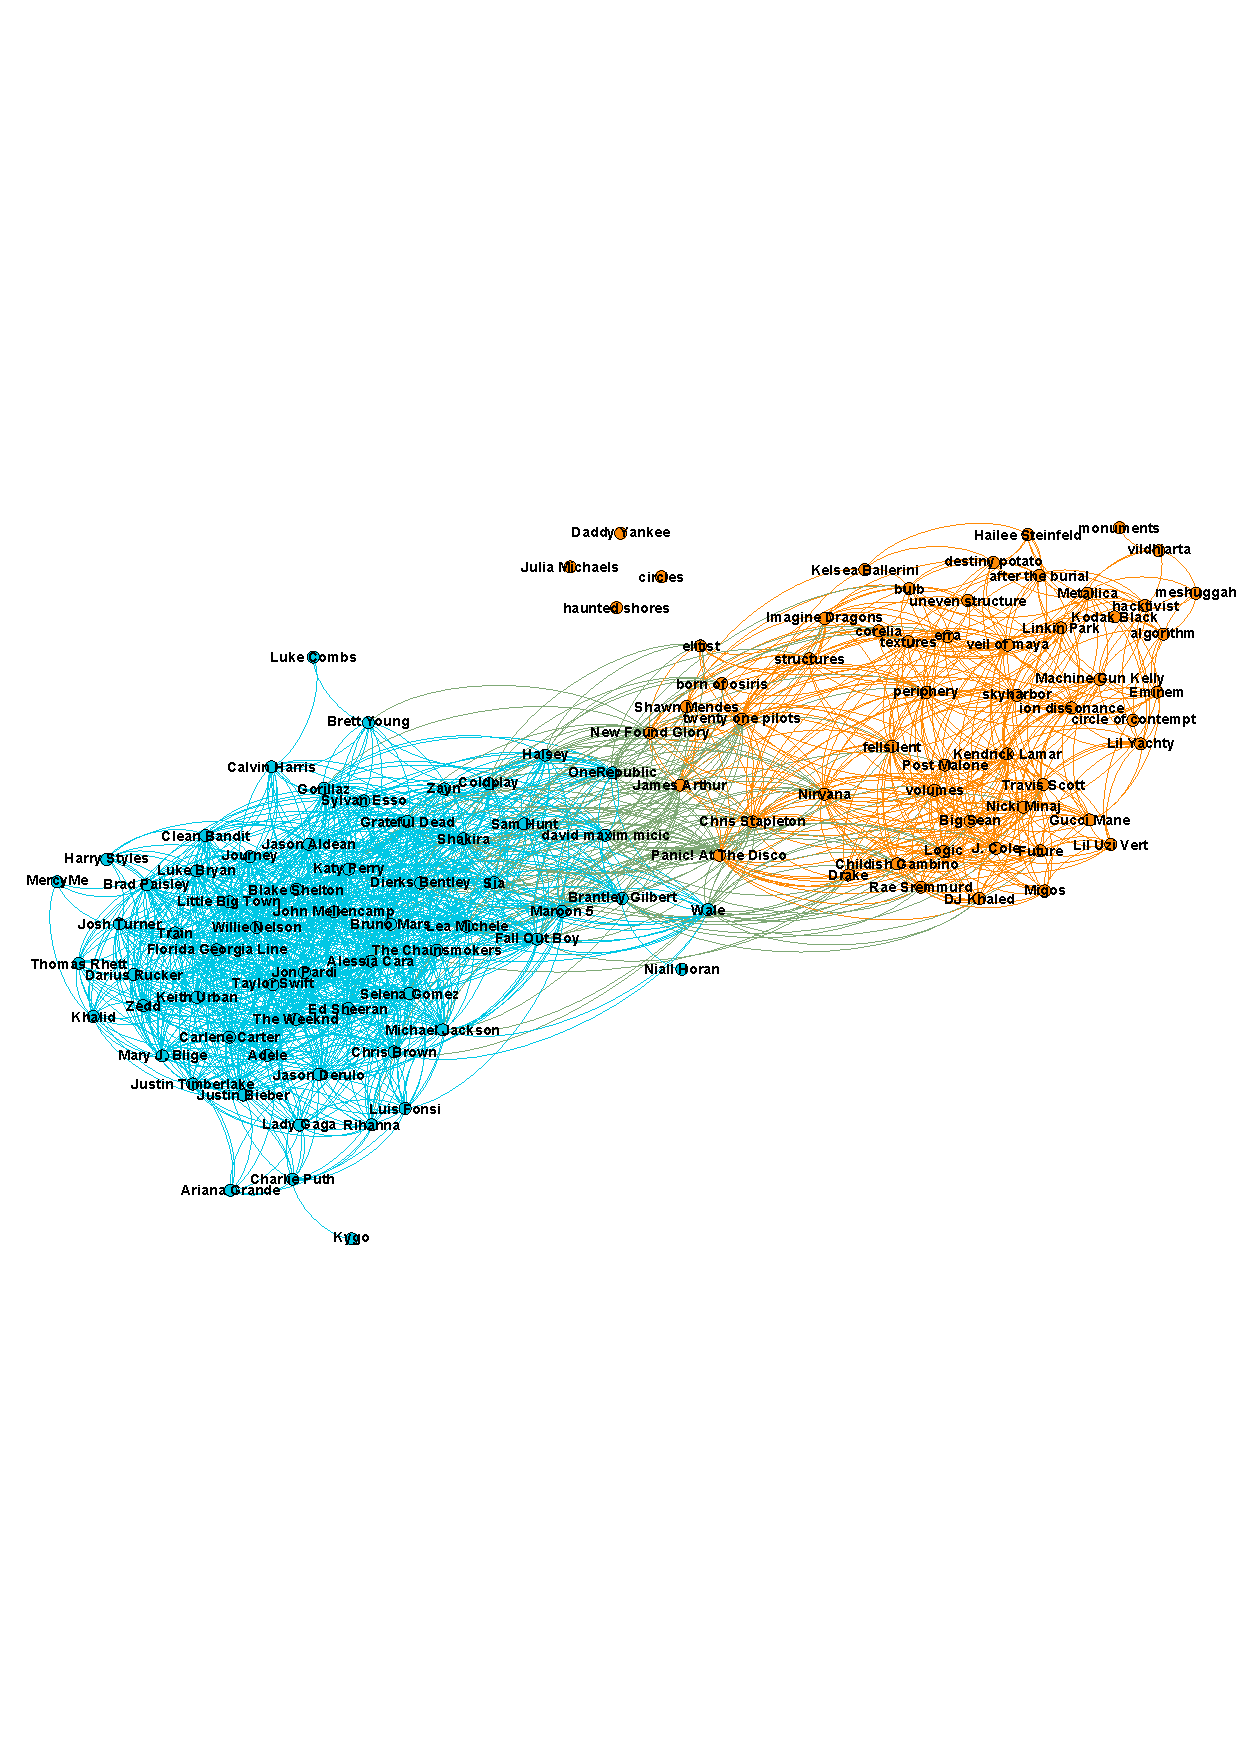
\includegraphics[trim=0mm 50mm 0mm 50mm, clip, width=0.7\linewidth]{data/emotion_similarity}
			\caption{Emotion similarity between artists}
			\label{fig:emotionsimilarity}
		\end{figure}
	
	\section{Topic Extraction}
	\label{sec:topicextraction}
	The Non-negative Matrix Factorization (NMF) algorithm has been used to extract potential topics from the lyrics. The \textit{sklearn} Python package provides everything necessary to apply NMF to the data. First, a tf-idf feature vector for each song text is calculated. Afterwards, these are fed into the NMF algorithm, which returns two matrices that...
	
	We found that a number of ten topics is appropriate for our dataset. When choosing more topics, they start to overlap too much. When choosing fewer topics, too much information is put into every single topic. This is of course subject to the experimentalist's taste.
	
		\subsection{Results}
		%Picture is not fully contained in pdf exported from Gephi
		%Need to do it again when I'm in the mood for it
		
		\begin{figure}[htb]
			\centering
			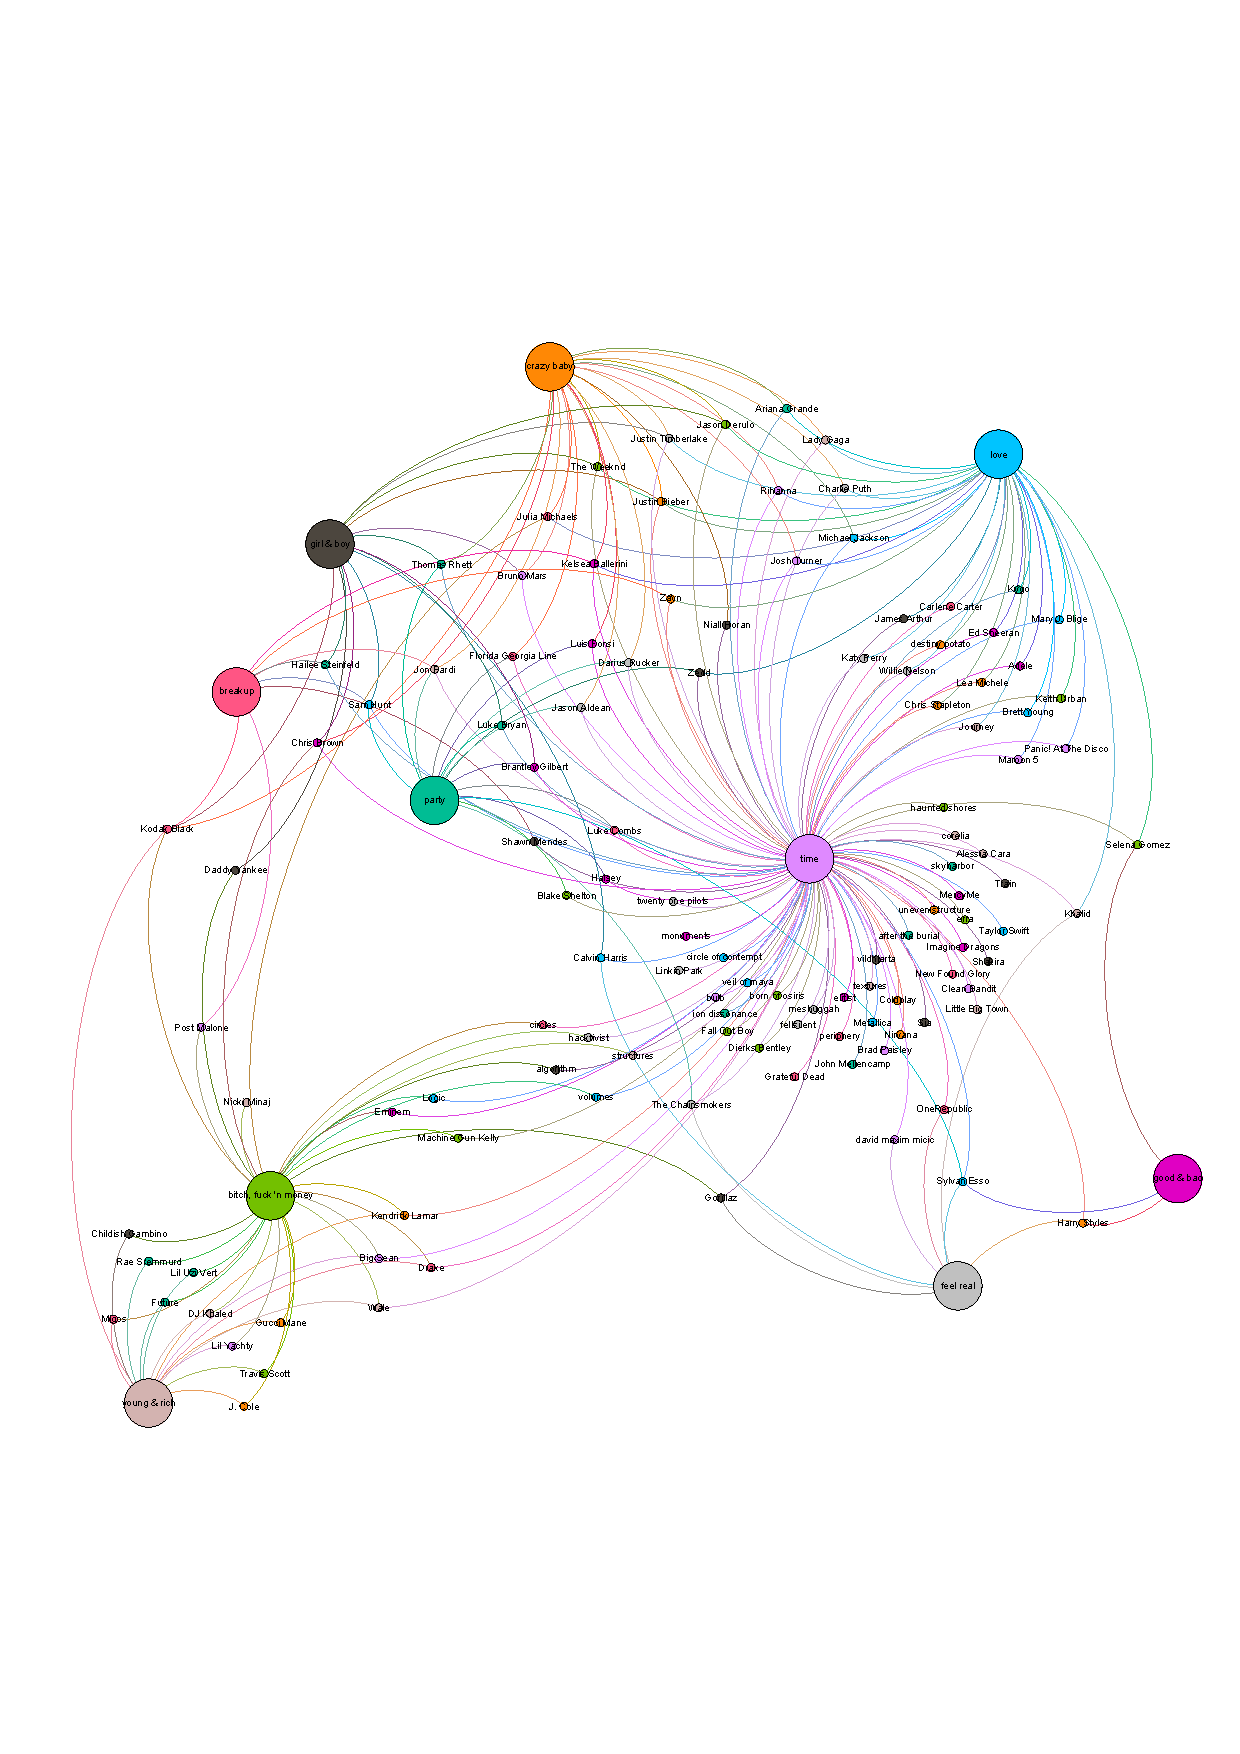
\includegraphics[trim=0mm 70mm 0mm 50mm, clip, width=\linewidth]{data/topic_graph}
			\caption{Full topic graph}
			\label{fig:topicgraph}
		\end{figure}
		
		\begin{figure}[htb]
			\centering
			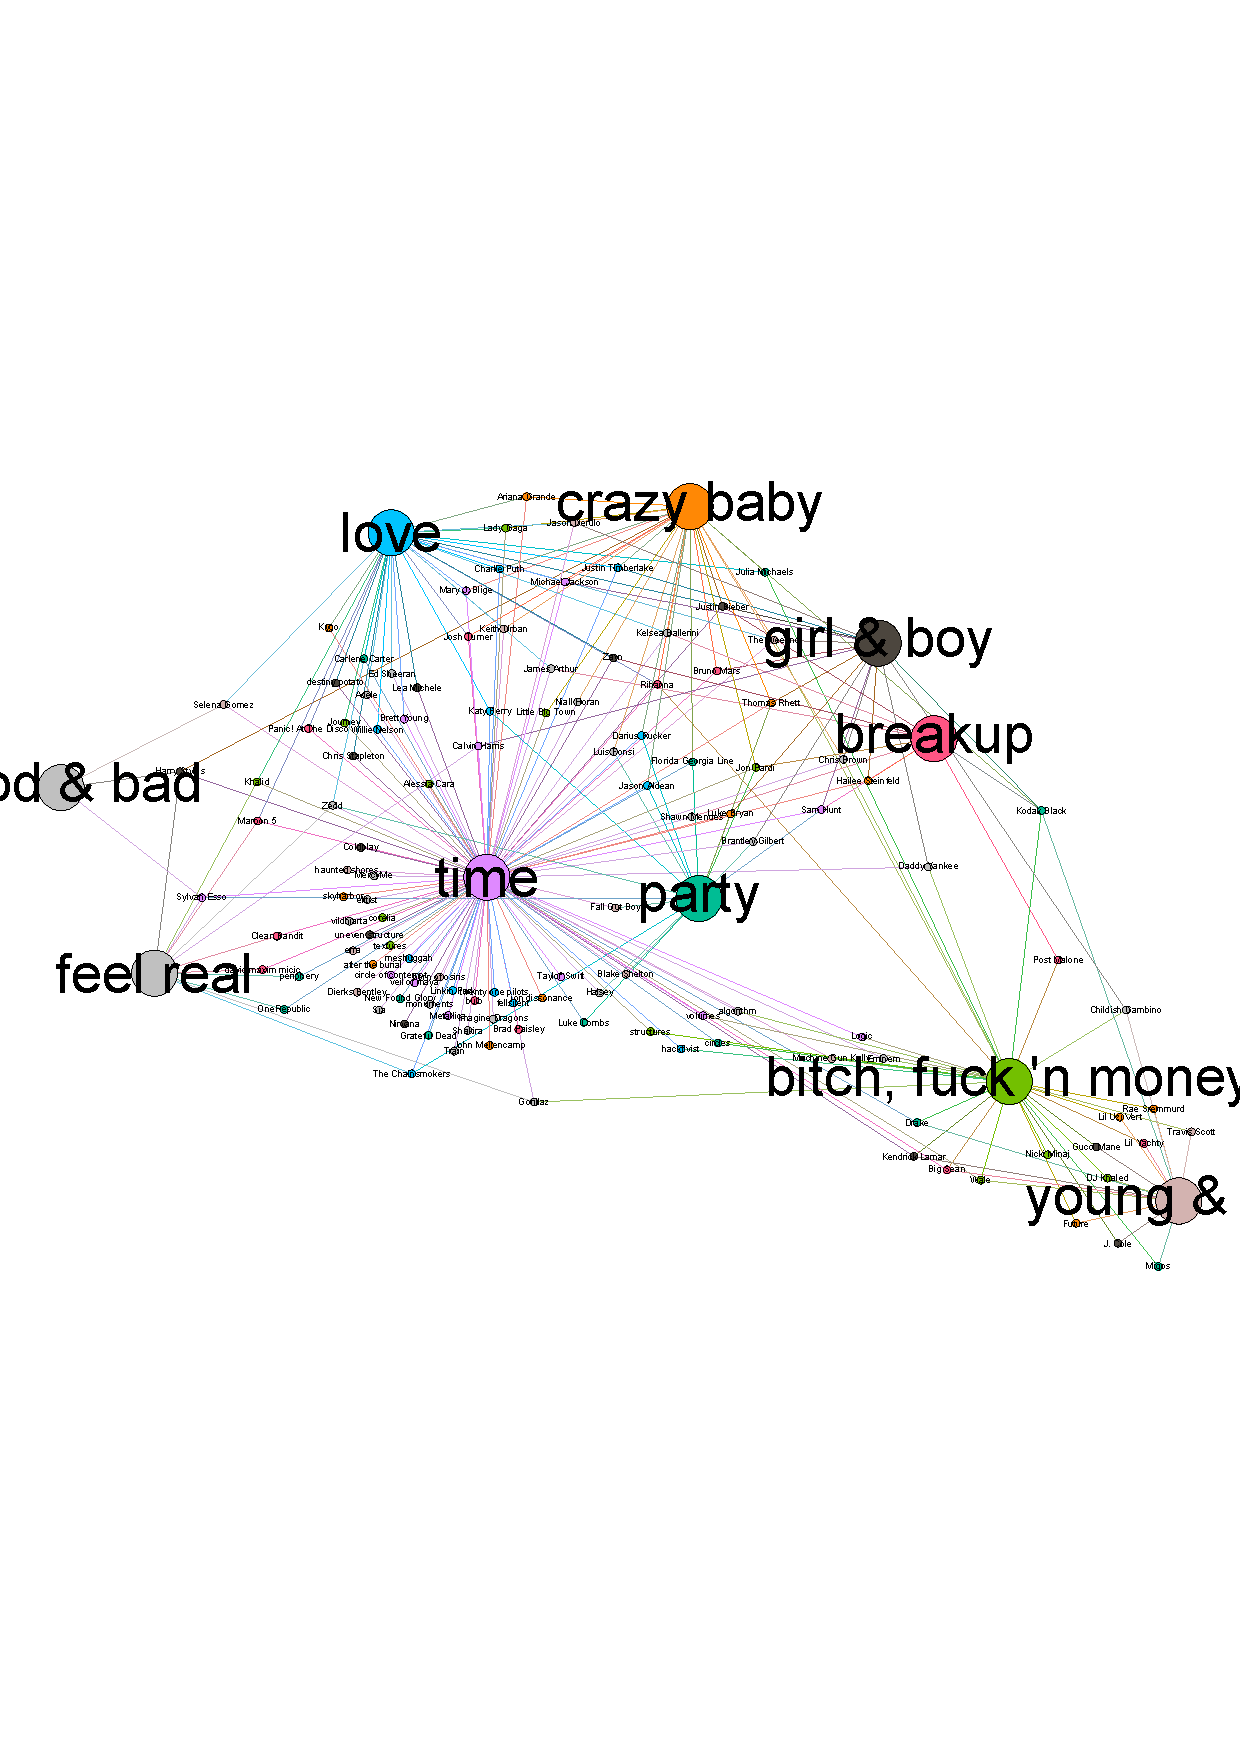
\includegraphics[trim=0mm 70mm 0mm 50mm, width=0.7\linewidth]{data/topic_graph_weight3-10}
			\caption{Topic graph with edge weights higher than $0.3$}
			\label{fig:reducedtopicgraph}
		\end{figure}
		
		\begin{figure}[htb]
			\centering
			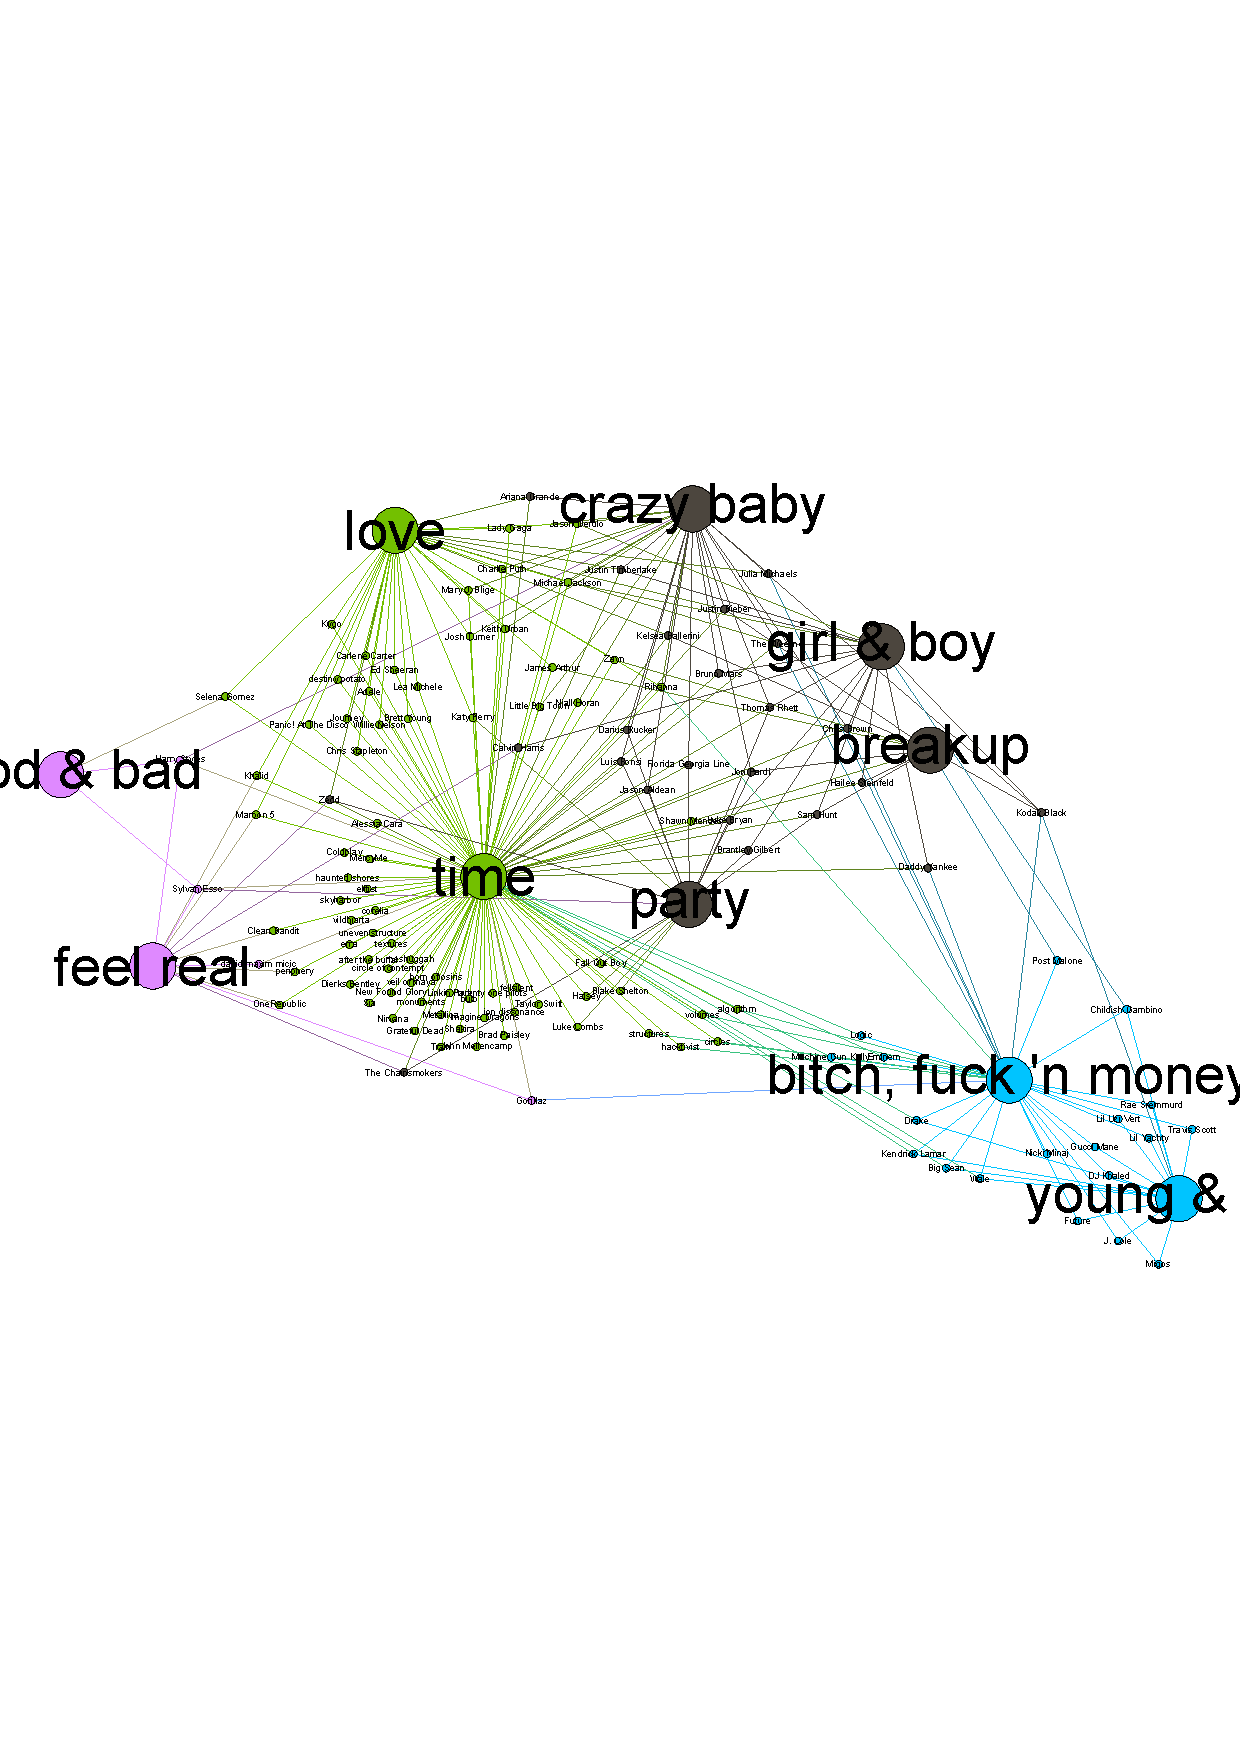
\includegraphics[trim=0mm 50mm 0mm 50mm, clip, width=0.7\linewidth]{data/topic_graph_new_modularity}
			\caption{Reduced topic graph with recalculated modularity}
			\label{fig:topicnewmod}
		\end{figure}
		
		Figure \ref{fig:topicsimilarity} shows the similarity of topics between artists. It is interesting to see that a lot of the rappers form their own subgraph, that is completely isolated from the rest of the graph.
		
		\begin{figure}[htb]
			\centering
			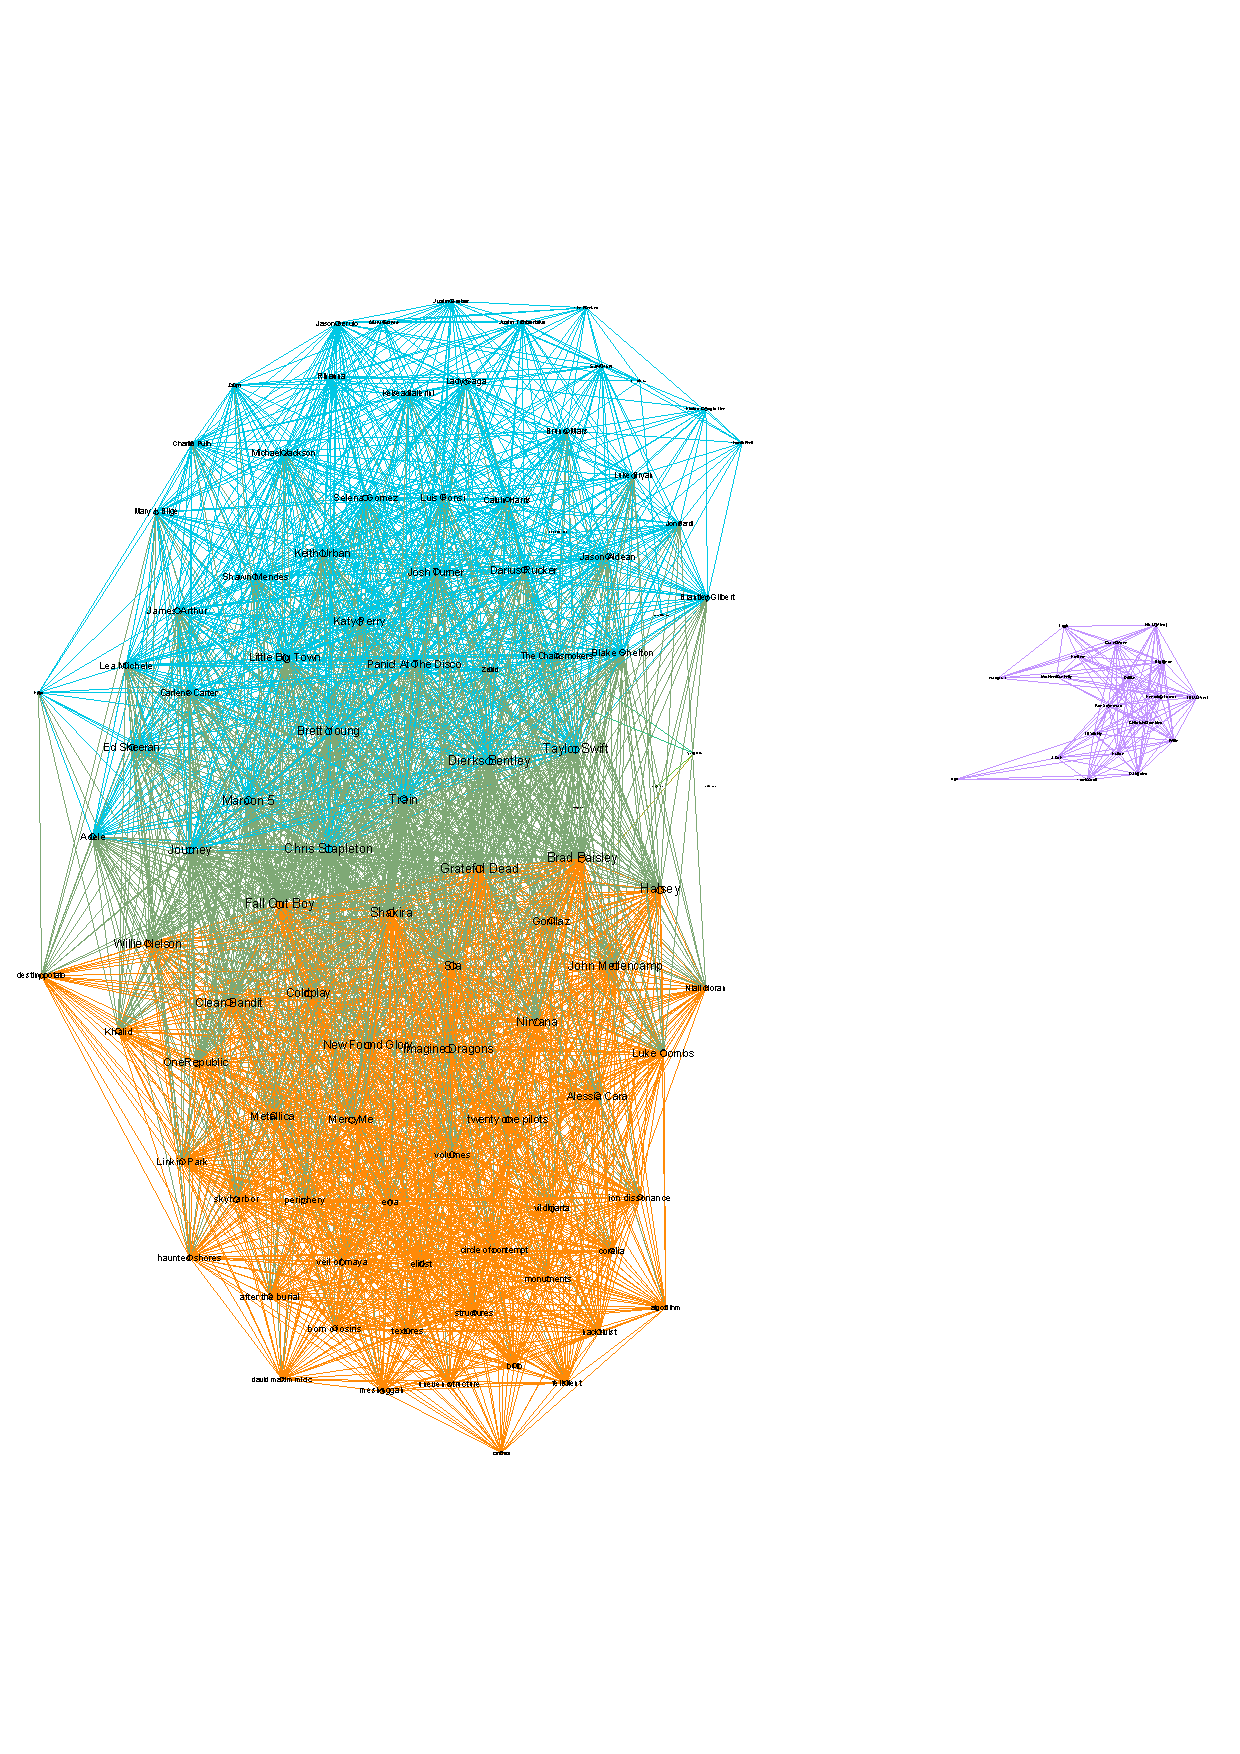
\includegraphics[trim=0mm 50mm 0mm 50mm, clip, width=\linewidth]{data/topic_similarity}
				\caption{Topic similarity between artists}
				\label{fig:topicsimilarity}
		\end{figure}
		
		\subsection{Evaluation}
		We tried to evaluate the resulting topics via held-out tests.
	
	\section{Other techniques}
	\label{sec:othertechniques}
	In this section we want to mention some of the techniques we used that were neglected as we settled for the approach we took in the end.
	POS Tagging
	Named Entity Extraction
	RAKE
	Summarization
	Text statistics (Flesch Score, etc.)

	\section{Conclusion}
	\label{sec:conclusion}
	
	\newpage
	
	\bibliography{rp}
	\bibliographystyle{apacite}
	
\end{document}